
In this chapter, we propose two new methods for estimating any sample quantile $\theta_q$ of the true extinction date, given a set of fossils. Both of these methods use test-statistic inversion: we first describe a novel approach called MINMI, which directly inverts a minimum statistic to estimate a quantile; then we describe SI-RM, an application of the the Robbins-Monro process, which can be considered a stochastic approximation extension of the simulated inversion estimator. 

\section{Minimum-Statistic Inversion (MINMI) Estimator}\label{new-method}

The MINMI\footnote{The name MINMI is a reference to \textit{Minmi Paravertebra}, a species of ankylosaur (or armoured dinosaur). Notably, \textit{Minmi} is the only known genus of ankylosaur from Australia, and was found in north-central Queensland \cite{Carpenter2001}. They were herbivores!} estimator assumes fossil recovery is uniformly distributed and that the distribution of measurement errors is known with constant variance. Then, using these assumptions, we are able to directly construct a quantile estimator by inversion.

\subsection{No Measurement Error Scenario}

Under the \hyperref[model: no-measurement-error]{$\delta$-model} proposed in \autoref{section: delta-model}, our fossil ages $X_i$ are uniform over $[\theta, K]$. Hence, we can compute the quantile function of the test-statistic $S(\bm{X})$ directly. Let the test statistic $S(\bm{X})$ be the MLE, the minimum statistic, and let $m$ denote the observed minimum value of $S(\bm{X})$:
\[
    \PP_\theta (S(\bm{X}) \geq m) = \prod_{i=1}^n \PP_\theta (X_i \geq m) = \left[ \PP_\theta (X_i \geq m) \right]^n = \left( \frac{K - m}{K - \theta} \right)^n
\]
\clearpage
Applying test-statistic inversion as per \autoref{eq: inversion}, we have
\begin{align*}\label{eq:minmi-no-measurement-error}
    q &= \PP_{\hat{\theta}_q}(S(\bm{X} \geq m) = \left( \frac{K - m}{K - \hat{\theta}_q} \right)^n \\
    \therefore \hat{\theta}_q &= K - q^{-1/n} (K-m) \numberthis
\end{align*}

where $\hat\theta_q$ is the MINMI estimate of $\theta_q$, such that $\PP_{\theta_q} (S(\bm{X}) \geq m) = q$.

\subsection{Measurement Error Scenario}

Let us next consider a scenario where measurement error is substantial. Under the \hyperref[model: measurement-error]{$\varepsilon$-model} proposed in \autoref{section: varepsilon-model}, we have conditionally uniform fossil ages $\bm{X|\varepsilon}$ and measurement error $\bm{\varepsilon}$ that are i.i.d with constant variance $\sigma^2$.

Consider the joint density of $(X, \varepsilon)$:
\[
    f_{X, \varepsilon} ( x , \varepsilon) = c f_{X | \varepsilon} ( x | \varepsilon=e) f(e)
\] where $x > \theta$, $x+e \leq K$, and $c$ is a normalising constant. Rearranging to find $c$:
\begin{align*}
    c^{-1}
        &= \int_{-\infty}^{K-\theta} \int_{\theta}^{K-e} f_{X | \varepsilon} ( x | \varepsilon=e) f(e) dx de\\
        &= \int_{-\infty}^{K-\theta} f(e) de \\
    \therefore c^{-1} &= F(K - \theta)
\end{align*}
where $F(y)=\int_{-\infty}^{y} f(e) de$ is the CDF of the measurement error.

Thus our joint density function is given by
\begin{align*}
    f_{X, \varepsilon} ( x , \varepsilon)
        =& [F(K - \theta)]^{-1} f_{X | \varepsilon} ( x | \varepsilon=e) f(e) \\
        =& [F(K - \theta)]^{-1} \frac{1}{K - e - \theta} f(e)
\end{align*}
since $X_i | \varepsilon_i \sim \mathcal{U}(\theta, K-\varepsilon_i)$. 

From this, we can geometrically identify our region of interest for finding $\PP_\theta ( X + \varepsilon \geq w)$, indicated by the shaded region in \autoref{fig: minmi_integral}.
\begin{figure}[ht]
    \centering
    % Created by tikzDevice version 0.12.3.1 on 2022-11-18 13:23:06
% !TEX encoding = UTF-8 Unicode
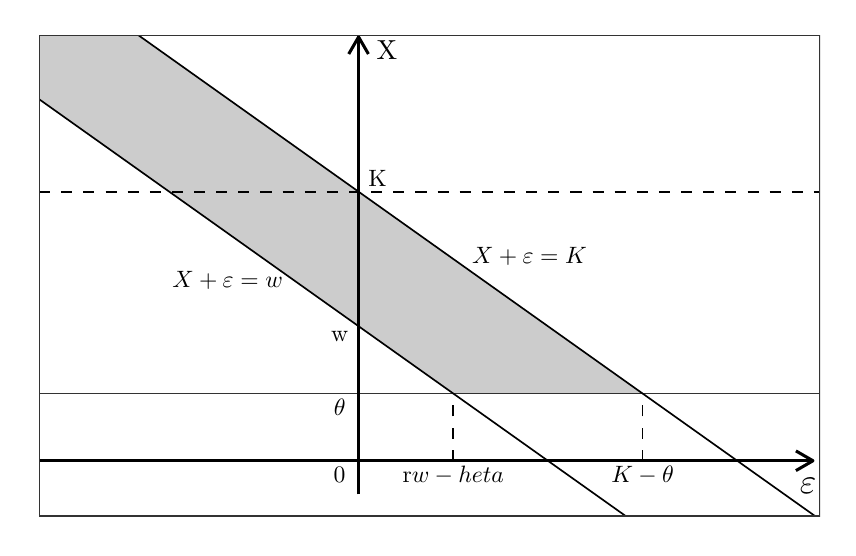
\begin{tikzpicture}[node distance = 2cm, auto, scale=0.5, transform shape, x=1pt,y=1pt]
\definecolor{fillColor}{RGB}{255,255,255}
\path[use as bounding box,fill=fillColor,fill opacity=0.00] (0,0) rectangle (578.16,361.35);
\begin{scope}
\path[clip] (  0.00,  0.00) rectangle (578.16,361.35);
\definecolor{drawColor}{RGB}{255,255,255}
\definecolor{fillColor}{RGB}{255,255,255}

\path[draw=drawColor,line width= 0.6pt,line join=round,line cap=round,fill=fillColor] (  0.00,  0.00) rectangle (578.16,361.35);
\end{scope}
\begin{scope}
\path[clip] (  8.25,  8.25) rectangle (572.66,355.85);
\definecolor{fillColor}{RGB}{255,255,255}

\path[fill=fillColor] (  8.25,  8.25) rectangle (572.66,355.85);
\definecolor{drawColor}{RGB}{0,0,0}

\path[draw=drawColor,line width= 1.1pt,line join=round] (-444.99, 48.36) -- (567.53, 48.36);

\path[draw=drawColor,line width= 1.1pt,line join=round] (555.21, 41.24) --
	(567.53, 48.36) --
	(555.21, 55.47);

\path[draw=drawColor,line width= 1.1pt,line join=round] (239.14, 24.05) -- (239.14,354.63);

\path[draw=drawColor,line width= 1.1pt,line join=round] (246.26,342.31) --
	(239.14,354.63) --
	(232.03,342.31);

\node[text=drawColor,anchor=base,inner sep=0pt, outer sep=0pt, scale=  1.99] at (259.67,338.05) {X};

\node[text=drawColor,anchor=base,inner sep=0pt, outer sep=0pt, scale=  2.56] at (564.11, 24.95) {$\varepsilon$};

\path[draw=drawColor,line width= 0.6pt,line join=round] (-556.16,807.97) -- (1137.07,-395.26);

\path[draw=drawColor,line width= 0.6pt,line join=round] (-556.16,710.74) -- (1137.07,-492.49);
\definecolor{fillColor}{RGB}{0,0,0}

\path[fill=fillColor,fill opacity=0.20] (-444.99,728.97) --
	(-438.15,724.11) --
	(-431.31,719.25) --
	(-424.46,714.39) --
	(-417.62,709.53) --
	(-410.78,704.67) --
	(-403.94,699.80) --
	(-397.10,694.94) --
	(-390.26,690.08) --
	(-383.42,685.22) --
	(-376.57,680.36) --
	(-369.73,675.50) --
	(-362.89,670.63) --
	(-356.05,665.77) --
	(-349.21,660.91) --
	(-342.37,656.05) --
	(-335.53,651.19) --
	(-328.69,646.33) --
	(-321.84,641.47) --
	(-315.00,636.60) --
	(-308.16,631.74) --
	(-301.32,626.88) --
	(-294.48,622.02) --
	(-287.64,617.16) --
	(-280.80,612.30) --
	(-273.95,607.43) --
	(-267.11,602.57) --
	(-260.27,597.71) --
	(-253.43,592.85) --
	(-246.59,587.99) --
	(-239.75,583.13) --
	(-232.91,578.27) --
	(-226.07,573.40) --
	(-219.22,568.54) --
	(-212.38,563.68) --
	(-205.54,558.82) --
	(-198.70,553.96) --
	(-191.86,549.10) --
	(-185.02,544.23) --
	(-178.18,539.37) --
	(-171.33,534.51) --
	(-164.49,529.65) --
	(-157.65,524.79) --
	(-150.81,519.93) --
	(-143.97,515.07) --
	(-137.13,510.20) --
	(-130.29,505.34) --
	(-123.45,500.48) --
	(-116.60,495.62) --
	(-109.76,490.76) --
	(-102.92,485.90) --
	(-96.08,481.03) --
	(-89.24,476.17) --
	(-82.40,471.31) --
	(-75.56,466.45) --
	(-68.71,461.59) --
	(-61.87,456.73) --
	(-55.03,451.87) --
	(-48.19,447.00) --
	(-41.35,442.14) --
	(-34.51,437.28) --
	(-27.67,432.42) --
	(-20.83,427.56) --
	(-13.98,422.70) --
	( -7.14,417.83) --
	( -0.30,412.97) --
	(  6.54,408.11) --
	( 13.38,403.25) --
	( 20.22,398.39) --
	( 27.06,393.53) --
	( 33.90,388.67) --
	( 40.75,383.80) --
	( 47.59,378.94) --
	( 54.43,374.08) --
	( 61.27,369.22) --
	( 68.11,364.36) --
	( 74.95,359.50) --
	( 81.79,354.63) --
	( 88.64,349.77) --
	( 95.48,344.91) --
	(102.32,340.05) --
	(109.16,335.19) --
	(116.00,330.33) --
	(122.84,325.47) --
	(129.68,320.60) --
	(136.52,315.74) --
	(143.37,310.88) --
	(150.21,306.02) --
	(157.05,301.16) --
	(163.89,296.30) --
	(170.73,291.43) --
	(177.57,286.57) --
	(184.41,281.71) --
	(191.26,276.85) --
	(198.10,271.99) --
	(204.94,267.13) --
	(211.78,262.27) --
	(218.62,257.40) --
	(225.46,252.54) --
	(232.30,247.68) --
	(239.14,242.82) --
	(245.99,237.96) --
	(252.83,233.10) --
	(259.67,228.23) --
	(266.51,223.37) --
	(273.35,218.51) --
	(280.19,213.65) --
	(287.03,208.79) --
	(293.88,203.93) --
	(300.72,199.07) --
	(307.56,194.20) --
	(314.40,189.34) --
	(321.24,184.48) --
	(328.08,179.62) --
	(334.92,174.76) --
	(341.76,169.90) --
	(348.61,165.03) --
	(355.45,160.17) --
	(362.29,155.31) --
	(369.13,150.45) --
	(375.97,145.59) --
	(382.81,140.73) --
	(389.65,135.87) --
	(396.50,131.00) --
	(403.34,126.14) --
	(410.18,121.28) --
	(417.02,116.42) --
	(423.86,111.56) --
	(430.70,106.70) --
	(437.54,101.83) --
	(444.38, 96.97) --
	(444.38, 96.97) --
	(437.54, 96.97) --
	(430.70, 96.97) --
	(423.86, 96.97) --
	(417.02, 96.97) --
	(410.18, 96.97) --
	(403.34, 96.97) --
	(396.50, 96.97) --
	(389.65, 96.97) --
	(382.81, 96.97) --
	(375.97, 96.97) --
	(369.13, 96.97) --
	(362.29, 96.97) --
	(355.45, 96.97) --
	(348.61, 96.97) --
	(341.76, 96.97) --
	(334.92, 96.97) --
	(328.08, 96.97) --
	(321.24, 96.97) --
	(314.40, 96.97) --
	(307.56, 96.97) --
	(300.72,101.83) --
	(293.88,106.70) --
	(287.03,111.56) --
	(280.19,116.42) --
	(273.35,121.28) --
	(266.51,126.14) --
	(259.67,131.00) --
	(252.83,135.87) --
	(245.99,140.73) --
	(239.14,145.59) --
	(232.30,150.45) --
	(225.46,155.31) --
	(218.62,160.17) --
	(211.78,165.03) --
	(204.94,169.90) --
	(198.10,174.76) --
	(191.26,179.62) --
	(184.41,184.48) --
	(177.57,189.34) --
	(170.73,194.20) --
	(163.89,199.07) --
	(157.05,203.93) --
	(150.21,208.79) --
	(143.37,213.65) --
	(136.52,218.51) --
	(129.68,223.37) --
	(122.84,228.23) --
	(116.00,233.10) --
	(109.16,237.96) --
	(102.32,242.82) --
	( 95.48,247.68) --
	( 88.64,252.54) --
	( 81.79,257.40) --
	( 74.95,262.27) --
	( 68.11,267.13) --
	( 61.27,271.99) --
	( 54.43,276.85) --
	( 47.59,281.71) --
	( 40.75,286.57) --
	( 33.90,291.43) --
	( 27.06,296.30) --
	( 20.22,301.16) --
	( 13.38,306.02) --
	(  6.54,310.88) --
	( -0.30,315.74) --
	( -7.14,320.60) --
	(-13.98,325.47) --
	(-20.83,330.33) --
	(-27.67,335.19) --
	(-34.51,340.05) --
	(-41.35,344.91) --
	(-48.19,349.77) --
	(-55.03,354.63) --
	(-61.87,359.50) --
	(-68.71,364.36) --
	(-75.56,369.22) --
	(-82.40,374.08) --
	(-89.24,378.94) --
	(-96.08,383.80) --
	(-102.92,388.67) --
	(-109.76,393.53) --
	(-116.60,398.39) --
	(-123.45,403.25) --
	(-130.29,408.11) --
	(-137.13,412.97) --
	(-143.97,417.83) --
	(-150.81,422.70) --
	(-157.65,427.56) --
	(-164.49,432.42) --
	(-171.33,437.28) --
	(-178.18,442.14) --
	(-185.02,447.00) --
	(-191.86,451.87) --
	(-198.70,456.73) --
	(-205.54,461.59) --
	(-212.38,466.45) --
	(-219.22,471.31) --
	(-226.07,476.17) --
	(-232.91,481.03) --
	(-239.75,485.90) --
	(-246.59,490.76) --
	(-253.43,495.62) --
	(-260.27,500.48) --
	(-267.11,505.34) --
	(-273.95,510.20) --
	(-280.80,515.07) --
	(-287.64,519.93) --
	(-294.48,524.79) --
	(-301.32,529.65) --
	(-308.16,534.51) --
	(-315.00,539.37) --
	(-321.84,544.23) --
	(-328.69,549.10) --
	(-335.53,553.96) --
	(-342.37,558.82) --
	(-349.21,563.68) --
	(-356.05,568.54) --
	(-362.89,573.40) --
	(-369.73,578.27) --
	(-376.57,583.13) --
	(-383.42,587.99) --
	(-390.26,592.85) --
	(-397.10,597.71) --
	(-403.94,602.57) --
	(-410.78,607.43) --
	(-417.62,612.30) --
	(-424.46,617.16) --
	(-431.31,622.02) --
	(-438.15,626.88) --
	(-444.99,631.74) --
	cycle;

\path[] (-444.99,728.97) --
	(-438.15,724.11) --
	(-431.31,719.25) --
	(-424.46,714.39) --
	(-417.62,709.53) --
	(-410.78,704.67) --
	(-403.94,699.80) --
	(-397.10,694.94) --
	(-390.26,690.08) --
	(-383.42,685.22) --
	(-376.57,680.36) --
	(-369.73,675.50) --
	(-362.89,670.63) --
	(-356.05,665.77) --
	(-349.21,660.91) --
	(-342.37,656.05) --
	(-335.53,651.19) --
	(-328.69,646.33) --
	(-321.84,641.47) --
	(-315.00,636.60) --
	(-308.16,631.74) --
	(-301.32,626.88) --
	(-294.48,622.02) --
	(-287.64,617.16) --
	(-280.80,612.30) --
	(-273.95,607.43) --
	(-267.11,602.57) --
	(-260.27,597.71) --
	(-253.43,592.85) --
	(-246.59,587.99) --
	(-239.75,583.13) --
	(-232.91,578.27) --
	(-226.07,573.40) --
	(-219.22,568.54) --
	(-212.38,563.68) --
	(-205.54,558.82) --
	(-198.70,553.96) --
	(-191.86,549.10) --
	(-185.02,544.23) --
	(-178.18,539.37) --
	(-171.33,534.51) --
	(-164.49,529.65) --
	(-157.65,524.79) --
	(-150.81,519.93) --
	(-143.97,515.07) --
	(-137.13,510.20) --
	(-130.29,505.34) --
	(-123.45,500.48) --
	(-116.60,495.62) --
	(-109.76,490.76) --
	(-102.92,485.90) --
	(-96.08,481.03) --
	(-89.24,476.17) --
	(-82.40,471.31) --
	(-75.56,466.45) --
	(-68.71,461.59) --
	(-61.87,456.73) --
	(-55.03,451.87) --
	(-48.19,447.00) --
	(-41.35,442.14) --
	(-34.51,437.28) --
	(-27.67,432.42) --
	(-20.83,427.56) --
	(-13.98,422.70) --
	( -7.14,417.83) --
	( -0.30,412.97) --
	(  6.54,408.11) --
	( 13.38,403.25) --
	( 20.22,398.39) --
	( 27.06,393.53) --
	( 33.90,388.67) --
	( 40.75,383.80) --
	( 47.59,378.94) --
	( 54.43,374.08) --
	( 61.27,369.22) --
	( 68.11,364.36) --
	( 74.95,359.50) --
	( 81.79,354.63) --
	( 88.64,349.77) --
	( 95.48,344.91) --
	(102.32,340.05) --
	(109.16,335.19) --
	(116.00,330.33) --
	(122.84,325.47) --
	(129.68,320.60) --
	(136.52,315.74) --
	(143.37,310.88) --
	(150.21,306.02) --
	(157.05,301.16) --
	(163.89,296.30) --
	(170.73,291.43) --
	(177.57,286.57) --
	(184.41,281.71) --
	(191.26,276.85) --
	(198.10,271.99) --
	(204.94,267.13) --
	(211.78,262.27) --
	(218.62,257.40) --
	(225.46,252.54) --
	(232.30,247.68) --
	(239.14,242.82) --
	(245.99,237.96) --
	(252.83,233.10) --
	(259.67,228.23) --
	(266.51,223.37) --
	(273.35,218.51) --
	(280.19,213.65) --
	(287.03,208.79) --
	(293.88,203.93) --
	(300.72,199.07) --
	(307.56,194.20) --
	(314.40,189.34) --
	(321.24,184.48) --
	(328.08,179.62) --
	(334.92,174.76) --
	(341.76,169.90) --
	(348.61,165.03) --
	(355.45,160.17) --
	(362.29,155.31) --
	(369.13,150.45) --
	(375.97,145.59) --
	(382.81,140.73) --
	(389.65,135.87) --
	(396.50,131.00) --
	(403.34,126.14) --
	(410.18,121.28) --
	(417.02,116.42) --
	(423.86,111.56) --
	(430.70,106.70) --
	(437.54,101.83) --
	(444.38, 96.97);

\path[] (444.38, 96.97) --
	(437.54, 96.97) --
	(430.70, 96.97) --
	(423.86, 96.97) --
	(417.02, 96.97) --
	(410.18, 96.97) --
	(403.34, 96.97) --
	(396.50, 96.97) --
	(389.65, 96.97) --
	(382.81, 96.97) --
	(375.97, 96.97) --
	(369.13, 96.97) --
	(362.29, 96.97) --
	(355.45, 96.97) --
	(348.61, 96.97) --
	(341.76, 96.97) --
	(334.92, 96.97) --
	(328.08, 96.97) --
	(321.24, 96.97) --
	(314.40, 96.97) --
	(307.56, 96.97) --
	(300.72,101.83) --
	(293.88,106.70) --
	(287.03,111.56) --
	(280.19,116.42) --
	(273.35,121.28) --
	(266.51,126.14) --
	(259.67,131.00) --
	(252.83,135.87) --
	(245.99,140.73) --
	(239.14,145.59) --
	(232.30,150.45) --
	(225.46,155.31) --
	(218.62,160.17) --
	(211.78,165.03) --
	(204.94,169.90) --
	(198.10,174.76) --
	(191.26,179.62) --
	(184.41,184.48) --
	(177.57,189.34) --
	(170.73,194.20) --
	(163.89,199.07) --
	(157.05,203.93) --
	(150.21,208.79) --
	(143.37,213.65) --
	(136.52,218.51) --
	(129.68,223.37) --
	(122.84,228.23) --
	(116.00,233.10) --
	(109.16,237.96) --
	(102.32,242.82) --
	( 95.48,247.68) --
	( 88.64,252.54) --
	( 81.79,257.40) --
	( 74.95,262.27) --
	( 68.11,267.13) --
	( 61.27,271.99) --
	( 54.43,276.85) --
	( 47.59,281.71) --
	( 40.75,286.57) --
	( 33.90,291.43) --
	( 27.06,296.30) --
	( 20.22,301.16) --
	( 13.38,306.02) --
	(  6.54,310.88) --
	( -0.30,315.74) --
	( -7.14,320.60) --
	(-13.98,325.47) --
	(-20.83,330.33) --
	(-27.67,335.19) --
	(-34.51,340.05) --
	(-41.35,344.91) --
	(-48.19,349.77) --
	(-55.03,354.63) --
	(-61.87,359.50) --
	(-68.71,364.36) --
	(-75.56,369.22) --
	(-82.40,374.08) --
	(-89.24,378.94) --
	(-96.08,383.80) --
	(-102.92,388.67) --
	(-109.76,393.53) --
	(-116.60,398.39) --
	(-123.45,403.25) --
	(-130.29,408.11) --
	(-137.13,412.97) --
	(-143.97,417.83) --
	(-150.81,422.70) --
	(-157.65,427.56) --
	(-164.49,432.42) --
	(-171.33,437.28) --
	(-178.18,442.14) --
	(-185.02,447.00) --
	(-191.86,451.87) --
	(-198.70,456.73) --
	(-205.54,461.59) --
	(-212.38,466.45) --
	(-219.22,471.31) --
	(-226.07,476.17) --
	(-232.91,481.03) --
	(-239.75,485.90) --
	(-246.59,490.76) --
	(-253.43,495.62) --
	(-260.27,500.48) --
	(-267.11,505.34) --
	(-273.95,510.20) --
	(-280.80,515.07) --
	(-287.64,519.93) --
	(-294.48,524.79) --
	(-301.32,529.65) --
	(-308.16,534.51) --
	(-315.00,539.37) --
	(-321.84,544.23) --
	(-328.69,549.10) --
	(-335.53,553.96) --
	(-342.37,558.82) --
	(-349.21,563.68) --
	(-356.05,568.54) --
	(-362.89,573.40) --
	(-369.73,578.27) --
	(-376.57,583.13) --
	(-383.42,587.99) --
	(-390.26,592.85) --
	(-397.10,597.71) --
	(-403.94,602.57) --
	(-410.78,607.43) --
	(-417.62,612.30) --
	(-424.46,617.16) --
	(-431.31,622.02) --
	(-438.15,626.88) --
	(-444.99,631.74);
\definecolor{drawColor}{RGB}{0,0,0}

\path[draw=drawColor,draw opacity=0.80,line width= 0.6pt,line join=round] (  8.25, 96.97) -- (572.66, 96.97);
\definecolor{drawColor}{RGB}{0,0,0}

\path[draw=drawColor,line width= 0.6pt,dash pattern=on 4pt off 4pt ,line join=round] (  8.25,242.82) -- (572.66,242.82);

\path[draw=drawColor,line width= 0.6pt,dash pattern=on 4pt off 4pt ,line join=round] (307.56, 48.36) -- (307.56, 96.97);

\path[draw=drawColor,line width= 0.6pt,dash pattern=on 4pt off 4pt ,line join=round] (444.38, 48.36) -- (444.38, 96.97);

\node[text=drawColor,anchor=base,inner sep=0pt, outer sep=0pt, scale=  1.71] at (252.83,246.66) {K};

\node[text=drawColor,anchor=base,inner sep=0pt, outer sep=0pt, scale=  1.71] at (225.46, 81.37) {$\theta$};

\node[text=drawColor,anchor=base,inner sep=0pt, outer sep=0pt, scale=  1.71] at (225.46,134.85) {w};

\node[text=drawColor,anchor=base,inner sep=0pt, outer sep=0pt, scale=  1.71] at (225.46, 32.76) {0};

\node[text=drawColor,anchor=base,inner sep=0pt, outer sep=0pt, scale=  1.71] at (307.56, 32.76) {r{$w-	heta$}};

\node[text=drawColor,anchor=base,inner sep=0pt, outer sep=0pt, scale=  1.71] at (444.38, 32.76) {$K-\theta$};

\node[text=drawColor,anchor=base west,inner sep=0pt, outer sep=0pt, scale=  1.71] at (321.24,190.76) {$X + \varepsilon = K$};

\node[text=drawColor,anchor=base east,inner sep=0pt, outer sep=0pt, scale=  1.71] at (184.41,173.74) {$X + \varepsilon = w$};
\definecolor{drawColor}{gray}{0.20}

\path[draw=drawColor,line width= 0.6pt,line join=round,line cap=round] (  8.25,  8.25) rectangle (572.66,355.85);
\end{scope}
\end{tikzpicture}

    \vspace{-10mm}
    \caption{Sketch of the region over which an integral should be taken to find $\PP_\theta ( X + \varepsilon \geq w)$. This region is indicated by the shaded area bounded by  $X+\varepsilon = K$ and $X + \varepsilon = w$, where $X \in [\theta, K]$ and $\varepsilon <= K-\theta$.}
    \label{fig: minmi_integral}
\end{figure}

Hence, we can find $\PP_\theta ( X + \varepsilon \geq w)$ for some value $w$. \begin{align*}
    \PP_\theta ( X + \varepsilon \geq w)
        =& 1 - \PP_\theta ( X + \varepsilon < w) \\
        =& 1 - \int_{-\infty}^{w-\theta} \int_{\theta}^{w-e} f_{X, \varepsilon}(x, e) dx de \quad \text{by inspection} \\
        =& 1 - \int_{-\infty}^{w-\theta} \int_{\theta}^{w-e} \frac{1}{K - \theta - e} \frac{1}{F (K - \theta)} f(e) dx de \\
        =& 1 - \frac{1}{F (K-\theta)} \int_{-\infty}^{w-\theta} \frac{w - \theta - e }{K - \theta - e} f(e) de \\
    \therefore \PP_\theta ( X + \varepsilon \geq w) =& 1 - \frac{F(w-\theta)}{F(K - \theta)} \psi(\theta; w) \numberthis \label{eqn:minmi}
\end{align*}
where $\psi(\theta; w) =  \int^{w-\theta}_{-\infty} \frac{w - e - \theta}{K - e - \theta) } \frac{f(e)}{F(w-\theta)} de$.

As before, we let our statistic $S(\bm{W})$ be the minimum statistic, $m$ be the observed minimum, and take $\theta_q$ such that $\PP_{\theta_q} (S(\bm{W}) \geq m) = q$:
\begin{align*}
    \PP_{\theta_q} (S(\bm{W}) \geq m)
      &= \prod_{i=1}^n \PP_{\theta_q} (X_{i} + \varepsilon_i \geq m) \\
    \implies q &= \left[ 1 - \frac{F(m-\theta_q)}{F(K - \theta_q)} \psi(\theta_q; m)  \right]^n \\
    q^{\frac{1}{n}} &= 1 - \frac{F(m-\theta_q)}{F(K - \theta_q)} \psi(\theta_q; m) \numberthis \label{eqn: minmi-ee}
\end{align*}
The MINMI estimator $\hat\theta_q$ can be found using inversion by solving the above \autoref{eqn: minmi-ee} for $\theta_q = \hat\theta_q$. However, since $\psi$ does not simplify in general, we propose approximate it with a Monte Carlo integral using $B$ Monte Carlo samples from $f(e)$, resulting in the below MINMI estimating equation:
\begin{align*}
    q^{\frac{1}{n}} &= 1 - \frac{F(m - \theta_q)}{F(K - \theta_q)} \hat\psi_B(\theta_q; m); &\hat\psi_B(\theta_q; m) =  \frac{1}{B} \sum_{b=1}^B \frac{m-e_b-\hat\theta_q}{K-e_b-\theta_q} \numberthis \label{eqn: minmi-ee-mc}
\end{align*} where $e_b$ are drawn from $f(e_b)$ truncated at $m-\hat\theta_q$

\subsection{Stochastically Increasing Property}\label{subsec: stochastically-increasing}

Generating confidence intervals by inversion is conditional on $\PP_{\theta} (S(\bm{W}) \geq m)$ being stochastically increasing in $\theta$. Although we were unable to show theoretically that this condition is true in general, we expect that it will be in most practical instances, and have been able to show this numerically under a range of parameter settings. We have been able to show that $\PP_{\theta_q} (S(\bm{W}) \geq m)$ is stochastically increasing under two assumptions, as below.
\begin{restatable}{theorem}{MinmiStochIncr}\label{theorem: stoch-increasing}
    Under the \hyperref[model: measurement-error]{$\varepsilon$-model} specified in \autoref{section: varepsilon-model}, if the following assumptions are satisfied:
    \begin{enumerate}
        \item The density function $f$ is symmetric and uni-modal about mean 0.
        \item $f(2|m-\theta|) > f(K-\theta) \left(2 + \frac{K-\theta}{|m-\theta|} \right)$
    \end{enumerate}
    Then $\PP_{\theta} (S(\bm{W}) \geq m)$ is stochastically increasing in $\theta$.
\end{restatable}

The proof of \autoref{theorem: stoch-increasing} is provided in \autoref{apx:minmi-stoch-incr-proof}.

Assumption 1 in \autoref{theorem: stoch-increasing} is clearly satisfied when we use a normal distribution to simulate measurement error, as we do in this thesis. Assumption 2 is not true at all values of $\theta$ (for example, if we were to choose $\theta$ to be arbitrarily close to $K$). But such values of $\theta$ are not plausible -- recall that $K$ and $\theta$ are the endpoints of the time interval under consideration, and $m$ is the most recently observed fossil. Hence $m$ we expect to be much closer to $\theta$ than to $K$ in settings of practical interest. Further, $K-\theta$ will typically be very large relative to measurement error, meaning that $f(K-\theta)$ will be very small, relative to $f(2|m-\theta|)$.

\subsection{Selecting the number of Monte Carlo Samples}\label{subsec:minmi-mce-var}

As the number of Monte Carlo samples increases, the variance of the MINMI estimator can be expected to decrease at the cost of greater computation: however, we would like to determine a way to obtain a ``good" value for $B$.

Using the delta method, we found the limiting distribution of $\sqrt{B}(\hat\theta_q - \theta_q)$ (a full derivation of is given in \autoref{apx:minmi-asymptotics-proof}):
\begin{restatable}{theorem}{ChooseMinmiB}\label{theorem: delta-method-variance}
    Under the \hyperref[model: measurement-error]{$\varepsilon$-model}, the limiting distribution of the MINMI estimator $\hat\theta_q$ is approximately normal as $B \rightarrow \infty$
    \[
        \sqrt{B}(\hat\theta_q - \theta_q) \stackrel{D}{\rightarrow} \cN \left(0, \sigma^2_{\psi(\theta_q)} \left[ \frac{F(m-\theta_q)}{F(K-\theta_q)\hat{u}^\prime(\theta_q)} \right]^2 \right)
    \] where $\sigma^2_{\psi(\theta_q)} = \Var\left(\psi(\theta_q)\right)$, $\psi(\theta) =  \int^{m-\theta}_{-\infty} \frac{m - e - \theta}{K - e - \theta) } \frac{f(e)}{F(w-\theta)} de$, $F(e)$ is the CDF of $\varepsilon$, and $\hat{u}(\theta) = \frac{F(m-\theta)}{F(K-\theta)} \hat{\psi}(\theta) - 1 + q^{1/n}$.
\end{restatable}

We were able to verify this result numerically, and observed the variance estimated by the delta method in \autoref{theorem: delta-method-variance} to be accurate to within 15\% for $B > 100$. This was done by comparing the delta method variance estimate to the sample variance of 250 MINMI estimates, repeating this process for values of B up to 3500. We verified this result for both the upper and lower endpoints of a central $95\%$ confidence interval at different values of $B$.
\begin{figure}[ht]
    \centering
    \includesvg[inkscapelatex=false, width=0.7\linewidth]{figures/minmi-delta-method_variance.svg}
    \caption{Percentage difference of the variance estimated by the delta method and the variance found numerically as $B$ increases. Note that the x-axis is on a $\log$ scale. The area shaded in green represents the region where the variance is accurate within 15\%, which we observed for $B > 100$. The dashed line indicates $B=100$.}
    \label{fig: minmi-delta-method-variance}
\end{figure}

In practice, we are interested in the value of $B$ that results in an estimator with ``low" variance. Rearranging the variance expression in \autoref{theorem: delta-method-variance}:
\begin{align*}
    \Var(\hat\theta_q) &\approx \frac{1}{B}\sigma^2_{\psi(\theta_q)} \left[ \frac{F(m-\theta_q)}{F(K-\theta_q)\hat{u}^\prime(\theta_q)} \right]^2 \\
    \implies B &\approx \frac{1}{\Var(\hat\theta_q)}\sigma^2_{\psi(\theta_q)} \left[ \frac{F(m-\theta_q)}{F(K-\theta_q)\hat{u}^\prime(\theta_q)} \right]^2
\end{align*}
Suppose we would like estimates with Monte Carlo error variance that is no larger than some small value $A$. Let $B^*$ denote the number of Monte Carlo samples required to achieve this. Then,
\begin{equation}\label{eqn:minmi-optimal-b}
    B^* \approx \frac{1}{A}\sigma^2_{\psi(\theta_q)} \left[ \frac{F(m-\theta_q)}{F(K-\theta_q)\hat{u}^\prime(\theta_q)} \right]^2
\end{equation}
Note that we must approximate $\theta_q$ and $\sigma^2_{\psi(\theta_q)}$ as their true values are unknown. For our purposes, pilot estimates for each will suffice: for instance, $\theta_q$ can be estimated using the MINMI estimator under the $\delta$-model as per \autoref{eq:minmi-no-measurement-error}, and a Monte Carlo estimate of $\sigma^2_{\psi(\theta_q)}$ can be obtained using some pilot number of Monte Carlo samples, such as $B=100$. For this thesis, we aimed to find estimates with Monte Carlo error variance no more than 20\% of our assumed measurement error variation, setting $A = 0.2*\sigma^2$.

\section{Simulated Inversion - Robbins Monro Process (SI-RM)}

We now propose applying the Robbins-Monro (RM) process to the estimation of extinction times, motivated by an application of the RM process to construct confidence intervals by \citet{Garthwaite1992}. We relate this to the simulated inversion estimator proposed by \citet{Huang2019} and apply it to estimating extinction times. Although the RM process has not yet been used to search for extinction times or endpoints of confidence intervals in palaeobiology, it is a generally well used technique in other spaces \cite{Carpenter1999, Fisher2020, Fu2015}.

\subsection{The Robbins-Monro Process}

The RM process is a stochastic approximation algorithm originally designed to solve various root-finding problems. It was later adapted to a specific root-finding problem of the form \cite{Fu2015} \[
M(\theta) \overset{\text{def}}{=} \E_\theta H(\bm{W}) = \beta
\] where $H(\bm{W})$ is some function of random variables $\bm{W}$ and $\beta \in \R$. The objective of the RM process is to find a sequence $\{\theta_n\}$ that converges to a unique (local) optimum $\theta^*$ by using the recursion \cite{LlyodBotev2015}
\[ \theta_{i+1} = \theta_i - c_i \Big( H(\bm{W}_i) - \beta \Big) \]
where $c_i > 0$ is the step size. \citet{RobbinsMonro1951} showed that, under weak regularity conditions, this recursion converges in mean square to the optimum $\theta^*$. However, the step sizes $c_n$ must decrease according to conditions $\sum_nc_n^2 < \infty$ and $\sum_n c_n = \infty$.

\subsection{The SI-RM Estimator}

We propose an inversion-based method for constructing central $100(1-\alpha)\%$ confidence intervals for $\theta$, applying the implementation of the RM process developed by \citet{Garthwaite1992}. They adapted the original scheme by letting $M(\theta) = \PP_\theta(S(\bm{W} > S(\bm{w}))$ and $\beta = \alpha/2$ (for the lower endpoint of the confidence interval, and $1-\alpha/2$ for the upper endpoint) where $S(\bm{w})$ is a point estimator of $\theta$. This scheme is described for the lower endpoint as follows:
\begin{align*}
    M(\theta) \overset{\text{def}}{=} \PP(S(\bm{W} > S(\bm{w})) = \alpha/2
\end{align*}

\citet{Garthwaite1992} designed this method to construct confidence intervals assuming that a point estimate (for instance, the maximum likelihood estimator) can be easily obtained, although in principle any statistic could be used if it is stochastically increasing in $\theta$, and as such we use $S(\bm{w})$ as previously. Next, let $\hat\theta_{q; i}$ be the estimate of $\theta_q$ at step $i$ of the RM process, for the $q$\textsuperscript{th} quantile. At each step of the process, generate a resample $\bm{w}^* = [w_1^*, \dots, w_n^*]$ by setting $\theta = \hat\theta_{q; i}$. Then, the next estimate $\hat\theta_{q; i+1}$ can be found by the recursion
\begin{equation}\label{eqn: SIRM-recursion}
    \hat\theta_{q; i+1} = \hat\theta_{q; i} - c/i \left( \mathbbm{1}_{\{S(\bm{w^*}) \geq S(\bm{w})\}} - q \right)
\end{equation}
where $c$ is a constant step length and $\mathbbm{1}$ is the indicator function.

The resample step, where we simulate new data according to our simulation model by setting $\theta = \hat\theta_{q; i}$, is similar to the simulated inversion estimator proposed by \citet{Huang2019}. As such, the application of the RM process can be thought of as a variation of the simulated-inversion estimator, where stochastic approximation is used to converge to an optimal estimate of $\theta_q$.

The recursion in \autoref{eqn: SIRM-recursion} must be adapted for the uniformity assumption in Models \ref{model: no-measurement-error} and \ref{model: measurement-error}, since $\theta_q$ must be positive and less than $K$. We propose recursing on a transformation of $\hat\theta_{q; i}$, to allow step sizes to still be defined on $\R$ while enforcing $\hat\theta_{q;i} < K$. Let $\eta$ be the following transformation:\begin{equation}
    \eta(\theta) = K -\ln(K-\theta)
\end{equation}
Hence, the recursion in \autoref{eqn: SIRM-recursion} becomes:
\begin{equation}
    \eta(\hat\theta_{q; i+1}) = \eta(\hat\theta_{q; i}) - c_\eta/i \left( \mathbbm{1}_{\{S(\bm{w^*}) \geq S(\bm{w})\}} - q \right)
\end{equation}
where $c_\eta$ denotes a constant step length on the same scale as $\eta$.

Estimates based on the RM process are clearly advantageous when the function $M(\theta)$ is unknown or too complex to be directly inverted. An example of this is if the uniformity assumption is relaxed, as depending on the distribution of the fossils, $M(\theta)$ may potentially be too complex to apply a method similar to the MINMI estimator. 

However, there are still some disadvantages to the SI-RM estimator. The flexibility of this method means we may expect it to be slower than MINMI, which exploits our knowledge of the form of the quantile function $P_{\theta_q}(S(\bm{W})>S(\bm{w}))$ to directly find an estimate. This will be explored by simulation in the next chapter. Moreover, the flexibility also means the method must be \textit{tuned} for each problem on a case-by-case basis, as choices of step size, starting values, and stopping criteria all significantly impact the exactness of estimates.

\subsection{Choice of Step Size}

The choice of $c_\eta$ has a significant impact on the performance of the RM process: too large, and the algorithm may oscillate back and forth without approaching the optimum; too small (relative to the magnitude of the gradient), and the iterates may never move, preventing convergence.

The optimal step length (let this be $c^*$) is dependent on $M^\prime(\theta)$ \cite{LlyodBotev2015}, which is typically unknown. As such, \citet{Garthwaite1992} proposed an \textit{adaptive} step length where $c_i$ is proportional to the distance between the current estimate at iteration $i$ and the observed point estimate $S(\bm{w})$:
\begin{equation}
    c_{\eta; i} = k\Big[\eta(S(\bm{w})) - \eta(\theta_{q; i})\Big] \left( 2\mathbbm{1}_{\{q \geq 0.5\}} - 1 \right)
\end{equation}

where $k$ is a proportionality constant dependent on the distribution of $S(\bm{w})$.

In the absence of better information, \citet{Garthwaite1992} set the step length proportionality constant $k$ to twice the optimal value for the normal distribution: \[
k = 2/\left[z_q \phi(z_q) \right]
\]
The recommendation to double the optimal value for the normal distribution comes because the cost (in terms of impact to the variance) of underestimating $c^*$ is greater than the cost of overestimating it -- specifically, the variance of $\hat\theta_q$ can increase significantly when step sizes are too small.

However, \citet{LlyodBotev2015} found that the above step length proposed by \citet{Garthwaite1992} leads to variances that are 20-30\% greater than the lower bound of the RM variance. Hence, although we will use the adaptive step size scheme in the experiments in subsequent chapters, we recognise this is an area where improvements can potentially be made.

\subsection{Choice of Starting Values}

The starting values used to initiate the RM process also affect convergence -- if initial estimates are not in the neighbourhood of the true value then it may be difficult to converge quickly to the optimum. As a result, \citet{Garthwaite1992} suggested some heuristics for selecting appropriate starting values for the RM process.

They propose the ``percentile method" for selecting starting points, proceeding with the process as though these starting points were reached after $m$ steps. For a $100(1-\alpha/2)\%$ confidence interval, starting values are found by first generating $(4-\alpha)/\alpha$ resamples with $\theta = S(\bm{w})$. The starting values for the upper and lower endpoints are then provided by the second largest and second smallest resamples, respectively.

The number of steps to skip, $m$, is chosen as
\[
    m = \min \left\{ 50, 0.3(4-\alpha)/\alpha \right\}
\]
Although the Robbins-Monro process is robust to the choice of starting values, good starting values improve the rate of convergence. The robustness is because step sizes are proportional to the distance from the observed point estimate $S(\bm{w})$. However, step sizes tend to be disproportionately large early on in the search. As a result, if starting estimates are too far away, convergence may take very long as the step lengths tend to be disproportionately large early in the process and it is possible for the RM process to be ``lost" for some time before converging to the answer (see \autoref{fig:SI-RM-starting-values}, where one of the searches for the lower bound ``runs away" to -2{\small,}000 before stepping back up. 
\begin{figure}[ht]
    \centering
    \includesvg[inkscapelatex=false, width=\linewidth]{figures/SI-RM-starting-estimate-convergence.svg}
    \caption{Left: SI-RM searches for the lower endpoint of a 95\% confidence interval. Right: SI-RM searches for the upper endpoint. \textcolor{red}{Red} is the search with starting values chosen by Garthwaite \& Buckland's percentile method \cite{Garthwaite1992}. Each line is a separate RM process performed on the same simulated dataset with different starting values.}
    \label{fig:SI-RM-starting-values}
\end{figure}

\subsection{Selecting Stopping Criteria}\label{subsec:si-rm-stopping-criteria}

The standard error of estimates obtained by the SI-RM process naturally reduces as the number of steps increases at the cost of computation time. We would like to stop the process once our estimates have variance that is below a certain value. However, there is currently no universal stopping criteria, since we are unable to approximate the expected variance at the $i$\textsuperscript{th} step of the RM process. 

Consider the limiting variance of the $(i+1)$\textsuperscript{th} estimate, which can be found using the delta method \cite{Garthwaite1992}
\[
    \Var\{\eta(\hat\theta_{q; i+1})\} = \frac{\alpha/2 (1-\alpha/2) c^2}{i(2cg-1)}, \quad g = \left[ \frac{d}{d\theta}M(\theta) \right]_{\theta = \eta(\theta_q)}
\] 
In practice, neither $\frac{d}{d\theta}M(\theta)$ nor $\theta_q$ are known, so $\Var(\hat\theta_{q; i+1})$ cannot be calculated. Currently there is no universal stopping criteria for the RM process; \citet{Garthwaite1992} proposed a manual approach by inspection, allowing the RM process to iterate for some time, pausing and inspecting for convergence, then restarting if not converged. In our simulation studies, we will use the estimated quantile function from the SI estimator proposed by \citet{Huang2019}, estimating $\frac{d}{d\theta}M(\theta)$ by symmetric finite difference \cite{Fu2015} for the purpose of illustration.